% Template for PLoS
% Version 3.5 March 2018
%
% % % % % % % % % % % % % % % % % % % % % %
%
% -- IMPORTANT NOTE
%
% This template contains comments intended 
% to minimize problems and delays during our production 
% process. Please follow the template instructions
% whenever possible.
%
% % % % % % % % % % % % % % % % % % % % % % % 
%
% Once your paper is accepted for publication, 
% PLEASE REMOVE ALL TRACKED CHANGES in this file 
% and leave only the final text of your manuscript. 
% PLOS recommends the use of latexdiff to track changes during review, as this will help to maintain a clean tex file.
% Visit https://www.ctan.org/pkg/latexdiff?lang=en for info or contact us at latex@plos.org.
%
%
% There are no restrictions on package use within the LaTeX files except that 
% no packages listed in the template may be deleted.
%
% Please do not include colors or graphics in the text.
%
% The manuscript LaTeX source should be contained within a single file (do not use \input, \externaldocument, or similar commands).
%
% % % % % % % % % % % % % % % % % % % % % % %
%
% -- FIGURES AND TABLES
%
% Please include tables/figure captions directly after the paragraph where they are first cited in the text.
%
% DO NOT INCLUDE GRAPHICS IN YOUR MANUSCRIPT
% - Figures should be uploaded separately from your manuscript file. 
% - Figures generated using LaTeX should be extracted and removed from the PDF before submission. 
% - Figures containing multiple panels/subfigures must be combined into one image file before submission.
% For figure citations, please use "Fig" instead of "Figure".
% See http://journals.plos.org/plosone/s/figures for PLOS figure guidelines.
%
% Tables should be cell-based and may not contain:
% - spacing/line breaks within cells to alter layout or alignment
% - do not nest tabular environments (no tabular environments within tabular environments)
% - no graphics or colored text (cell background color/shading OK)
% See http://journals.plos.org/plosone/s/tables for table guidelines.
%
% For tables that exceed the width of the text column, use the adjustwidth environment as illustrated in the example table in text below.
%
% % % % % % % % % % % % % % % % % % % % % % % %
%
% -- EQUATIONS, MATH SYMBOLS, SUBSCRIPTS, AND SUPERSCRIPTS
%
% IMPORTANT
% Below are a few tips to help format your equations and other special characters according to our specifications. For more tips to help reduce the possibility of formatting errors during conversion, please see our LaTeX guidelines at http://journals.plos.org/plosone/s/latex
%
% For inline equations, please be sure to include all portions of an equation in the math environment.  For example, x$^2$ is incorrect; this should be formatted as $x^2$ (or $\mathrm{x}^2$ if the romanized font is desired).
%
% Do not include text that is not math in the math environment. For example, CO2 should be written as CO\textsubscript{2} instead of CO$_2$.
%
% Please add line breaks to long display equations when possible in order to fit size of the column. 
%
% For inline equations, please do not include punctuation (commas, etc) within the math environment unless this is part of the equation.
%
% When adding superscript or subscripts outside of brackets/braces, please group using {}.  For example, change "[U(D,E,\gamma)]^2" to "{[U(D,E,\gamma)]}^2". 
%
% Do not use \cal for caligraphic font.  Instead, use \mathcal{}
%
% % % % % % % % % % % % % % % % % % % % % % % % 
%
% Please contact latex@plos.org with any questions.
%
% % % % % % % % % % % % % % % % % % % % % % % %

\documentclass[10pt,letterpaper]{article}
\usepackage[top=0.85in,left=2.75in,footskip=0.75in]{geometry}

% amsmath and amssymb packages, useful for mathematical formulas and symbols
\usepackage{amsmath,amssymb}

% Use adjustwidth environment to exceed column width (see example table in text)
\usepackage{changepage}

% Use Unicode characters when possible
\usepackage[utf8x]{inputenc}

% textcomp package and marvosym package for additional characters
\usepackage{textcomp,marvosym}

% cite package, to clean up citations in the main text. Do not remove.
\usepackage{cite}

% Use nameref to cite supporting information files (see Supporting Information section for more info)
\usepackage{nameref,hyperref,comment}

% line numbers
\usepackage[right]{lineno}

% ligatures disabled
%\usepackage{microtype}
%\DisableLigatures[f]{encoding = *, family = * }

% color can be used to apply background shading to table cells only
\usepackage[table]{xcolor}

% array package and thick rules for tables
\usepackage{array}

% create "+" rule type for thick vertical lines
\newcolumntype{+}{!{\vrule width 2pt}}

% create \thickcline for thick horizontal lines of variable length
\newlength\savedwidth
\newcommand\thickcline[1]{%
  \noalign{\global\savedwidth\arrayrulewidth\global\arrayrulewidth 2pt}%
  \cline{#1}%
  \noalign{\vskip\arrayrulewidth}%
  \noalign{\global\arrayrulewidth\savedwidth}%
}

% \thickhline command for thick horizontal lines that span the table
\newcommand\thickhline{\noalign{\global\savedwidth\arrayrulewidth\global\arrayrulewidth 2pt}%
\hline
\noalign{\global\arrayrulewidth\savedwidth}}


% Remove comment for double spacing
%\usepackage{setspace} 
%\doublespacing

% Text layout
\raggedright
\setlength{\parindent}{0.5cm}
\textwidth 5.25in 
\textheight 8.75in

% Bold the 'Figure #' in the caption and separate it from the title/caption with a period
% Captions will be left justified
\usepackage[aboveskip=1pt,labelfont=bf,labelsep=period,justification=raggedright,singlelinecheck=off]{caption}
\renewcommand{\figurename}{Fig}

% Use the PLoS provided BiBTeX style
\bibliographystyle{plos2015}

% Remove brackets from numbering in List of References
\makeatletter
\renewcommand{\@biblabel}[1]{\quad#1.}
\makeatother



% Header and Footer with logo
\usepackage{lastpage,fancyhdr,graphicx}
\usepackage{epstopdf}
%\pagestyle{myheadings}
\pagestyle{fancy}
\fancyhf{}
%\setlength{\headheight}{27.023pt}
%\lhead{\includegraphics[width=2.0in]{PLOS-submission.eps}}
\rfoot{\thepage/\pageref{LastPage}}
\renewcommand{\headrulewidth}{0pt}
\renewcommand{\footrule}{\hrule height 2pt \vspace{2mm}}
\fancyheadoffset[L]{2.25in}
\fancyfootoffset[L]{2.25in}
\lfoot{\today}

%% Include all macros below

\newcommand{\FIRSTkit}{{\tt FIRSTkit }}
\newcommand{\R}{{\tt R }}

%% END MACROS SECTION


\begin{document}
\vspace*{0.2in}

% Title must be 250 characters or less.
\begin{flushleft}
{\Large
\textbf\newline{FIRSTkit: First Impressions R-based Statistics Toolkit} % Please use "sentence case" for title and headings (capitalize only the first word in a title (or heading), the first word in a subtitle (or subheading), and any proper nouns).
}
\newline
% Insert author names, affiliations and corresponding author email (do not include titles, positions, or degrees).
\\
Israel A. Almod\'ovar-Rivera \textsuperscript{1\ddag},
Ranjan Maitra \textsuperscript{2\ddag},
\\
\bigskip
\textbf{1} Department of Mathematical Sciences, University of Puerto Rico at Mayaguez Campus, Mayaguez, PR, USA
%\textbf{1} Department of Biostatistics and Epidemiology, University of Puerto Rico at Medical Science Campus, San Juan, PR, USA
\\
\textbf{2} Department of Statistics, Iowa State University, Ames, IA, USA
\\
\bigskip

% Insert additional author notes using the symbols described below. Insert symbol callouts after author names as necessary.
% 
% Remove or comment out the author notes below if they aren't used.
%
% Primary Equal Contribution Note
%\Yinyang These authors contributed equally to this work.

% Additional Equal Contribution Note
% Also use this double-dagger symbol for special authorship notes, such as senior authorship.
\ddag These authors also contributed equally to this work.

% Current address notes
\textcurrency Current Address: Department of Mathematical Sciences, University of Puerto Rico at Mayaguez Campus, Mayaguez, PR, USA
%\textcurrency Current Address: Department of Biostatistics and Epidemiology, University of Puerto Rico at Medical Science Campus, San Juan, PR, USA % change symbol to "\textcurrency a" if more than one current address note
% \textcurrency b Insert second current address 
% \textcurrency c Insert third current address

% Deceased author note
%\dag Deceased

% Group/Consortium Author Note
%\textpilcrow Membership list can be found in the Acknowledgments section.

% Use the asterisk to denote corresponding authorship and provide email address in note below.
*israel.almodovar@upr.edu

\end{flushleft}
% Please keep the abstract below 300 words
\section*{Abstract}

Something will be added here...
\linenumbers

% Use "Eq" instead of "Equation" for equation citations.
\section*{Introduction}

Modularity is a pervasive concept in computer science, extending from the design of systems (Parnas 1972), to the design of software (Szyperski 1996). Modularity offers several advantages to both a developer and a user. In particular, functionality can be dynamically loaded and unloaded depending on the particular use case. Open source modular software precipitates the possibility of extensions contributed by a wide array of programmers, which can allow the software to morph into areas that weren’t anticipated early in development. In the statistics realm, \R (\R Core Team 2014) is a prime example of the virtues of modular programming. As of this writing, The Comprehensive \R Archive Network (CRAN) contains over 9000 source packages which can be installed and dynamically loaded in a particular
session as needed.

Modern web technologies have enabled a new generation of software packages that reside solely on the web, which eliminates the issue of local installation and helps abstract away some of the more challenging programming aspects of working directly with \R. Upon the release of RStudio’s Shiny (RStudio and Inc. 2014) it became easier for an \R-based analysis to be converted to an interactive web application. Several recent software packages have built upon Shiny to provide a web-based system based on R. One such package is iNZight Lite (Wild 2015) which attempts to expose students to data analysis without requiring programming knowledge. Like most web-based systems, this does not include reproducible \R code, which limits its usefulness in a scientific or academic setting. Another package is called Radiant (Nijs 2016), which is a web-based application with the aim of furthering business education and financial analysis. While the application is modular and extensible, it does require installation and hosting and is inundated with more features than necessary for an introductory student.  Partial fulfillment of requirements is noted in the table, as well as a measure of the complexity of functionality offered by default. For example, \R does have an associated Graphical User Interface (GUI), however this interface is very limited, thus only partially fulfilling the behavior of a GUI.

Unlike other web-based application, \FIRSTkit is done with the purpose to be used as a teaching component.

As a statistician in a School of Public Health, I saw first hand students struggling with \R, either by the difficulty or just they weren't interested. The goal of \FIRSTkit is to allow first time {\tt R} users, or users who have low interest in learning coding in perform basic statistics.

As a web-based application, this tool is immediately more familiar to students than a desktop application. The need for dealing with software licenses, installation configuration, and supported platforms has been eliminated. This allows students to spend more time working with the data and learning statistics than having to struggle to get the software running.

Unlike paid softwares, \FIRSTkit requires no software licenses or manual installation. \FIRSTkit 'functionality is focused on introductory statistics students, and nothing more (no extraneous functionality that must be navigated around to get to the content they need). \FIRSTkit provides students an opportunity to see the underlying functionality of the buttons, text boxes, and other UI elements, in an attempt to foster an interest in coding.



\section*{\FIRSTkit capabilities}

The widespread adoption of \R as a tool for statistical analysis has undoubtedly been an important development for the scientific community. However, using \R in most cases still requires a basic knowledge of programming concepts which may pose a steep learning curve for the introductory statistics student (Tan, Ting, and Ling 2009). The website is organized around the idea in how introductory statistics courses are carry. \FIRSTkit capabilities are descriptive statistics, inference and regression. In terms of the descriptive statistics, the user can obtain location summaries as well dispersion. 

\subsection{Descriptive Statistics}

Describing (or summarizing) a data in a clear in a concise way is one of the first things we usually taught in a introductory statistics courses. Many methods are available for summarizing data in both numeric and graphical form. \FIRSTkit allow to obtain summary regarding location and dispersion. In terms of location these are sample mean, trimmed mean, median, and geometric mean. Given a sample of size $n$, consider independent random variables $X_1, X_2,\ldots, X_n$ that we wish to summarized. 

\subsubsection{Location Measurements}

\begin{figure}
  \centering
  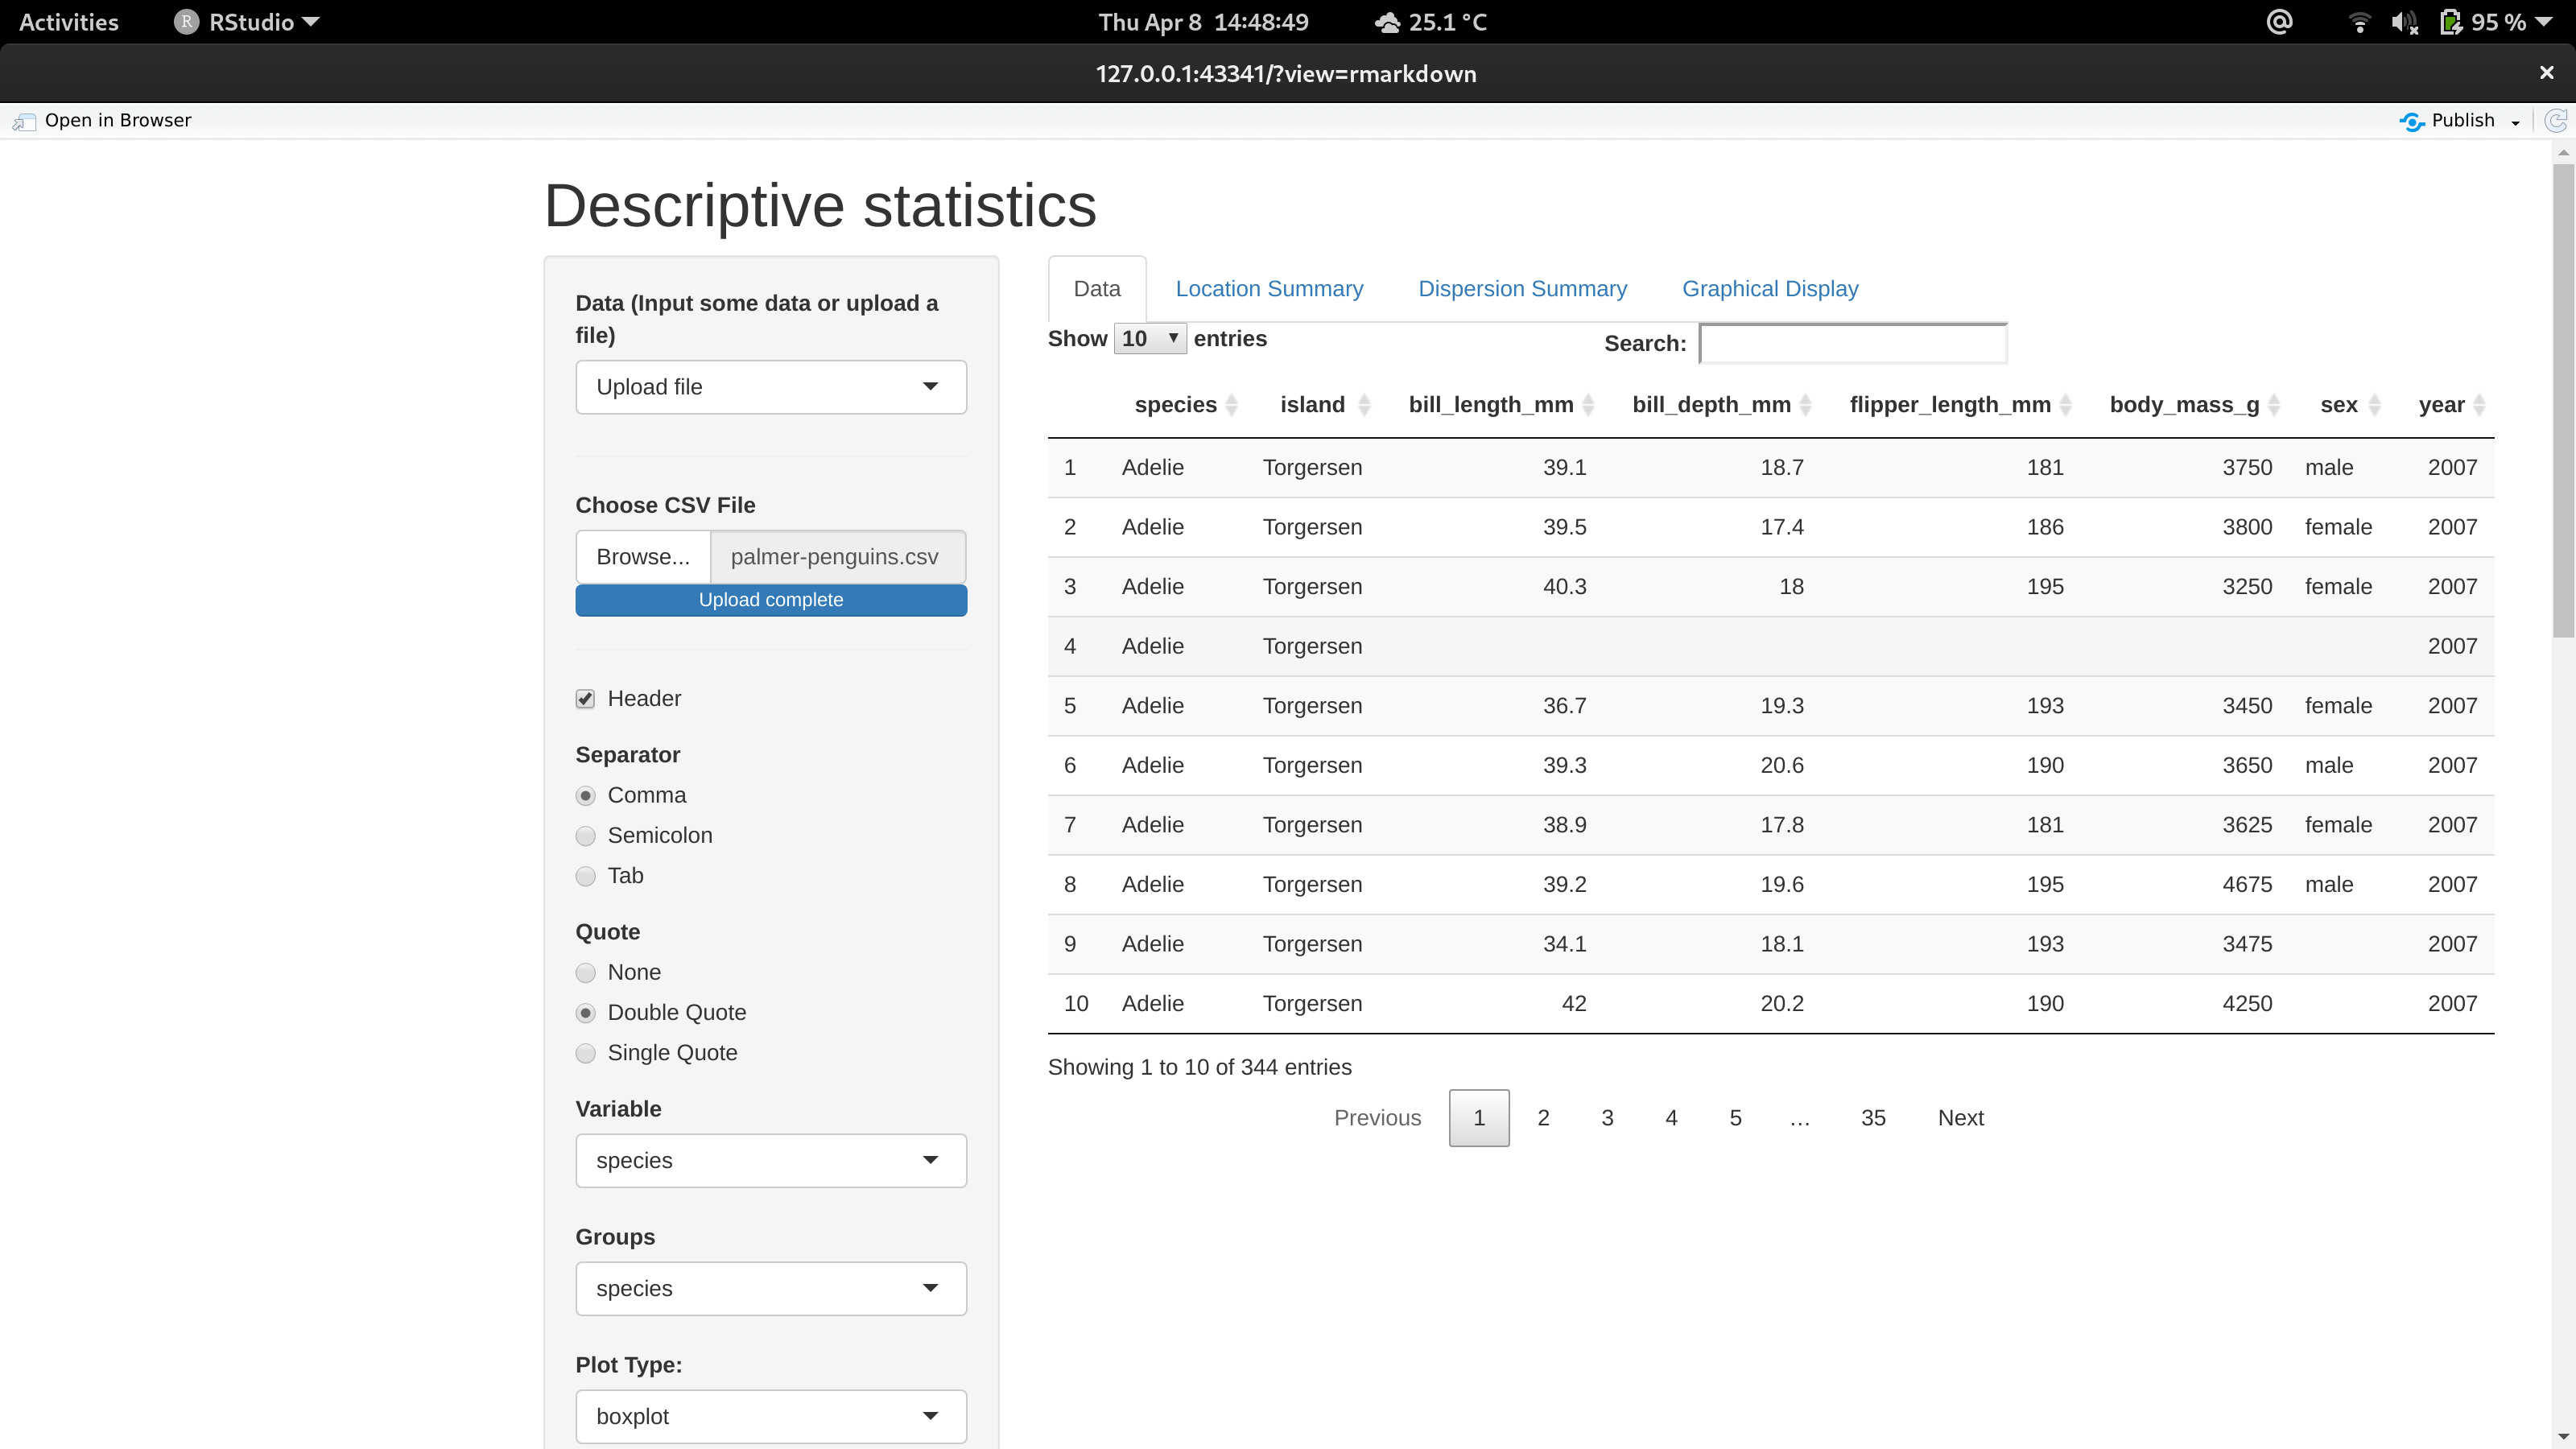
\includegraphics[width=\textwidth]{figures/Descriptive1}
  \end{figure}
\begin{enumerate}
\item {\bf Arithmetic mean}: The sample mean from a group of observations is an estimate of the population mean $\mu$.  The sample mean is defined to be,
\[
\bar{x}= \frac{1}{n}\sum^n_{i=1}x_i
\]
\item Trimmed mean: This mean is computed after discarding given parts of a probability distribution or sample at the high and low end, and typically discarding an equal amount of both. This number of points to be discarded is usually given as a percentage of the total number of points, but may also be given as a fixed number of points. 
\begin{enumerate}
\item First find $n =$ number of observations.
\item Reorder them as ``order statistic''' $X_i$ from the smallest to the largest.
\item Find lower case $p=P/100$ = proportion trimmed.
\item Compute $np$. If $np$ is an integer use $k=np$ and trim $k$ observations at both ends. $R = \mbox{remaining observations} = n-2k$. The trimmed mean is defined as,
\[
\bar{x}_{k} = \frac{X_{k+1}+X_{k+2}+\cdots+X_{n-k}}{R} 
\]
\end{enumerate}
\item Median: Middle value separating the greater and lesser halves of a data set ,
\[
M = X_{(0.5 \times n)}
\]
\item Geometric Mean: The geometric mean of a non-empty data set of (positive) numbers is always at most their arithmetic mean. Equality is only obtained when all numbers in the data set are equal; otherwise, the geometric mean is smaller. 
\[
g = \left(\prod^n_{i=1}x_i\right)^{1/n}
\]
\end{enumerate}


\subsection{Dispersion Measurements}
Given a sample of size $n$, consider  independent random variables $X_1, X_2,\ldots, X_n$, each corresponding to one randomly selected observation. Each of these variables has the distribution of the population, with mean $\mu$ and standard deviation $\sigma$.
\begin{enumerate}
\item Sample standard deviation: is a measure of the amount of variation or dispersion of a set of values.
\[
s = \sqrt{\frac{1}{n}\sum^n_{i=1}(x_i-\bar{x})^2}
\]
\item Sample Variance: is the expectation of the squared deviation of a random variable from its mean. Informally, it measures how far a set of numbers is spread out from their average value. 
\[
s^2 = \frac{1}{n}\sum^n_{i=1}(x_i-\bar{x})^2
\]
\item Interquartile Range:  difference between 75th and 25th percentiles, or between upper and lower quartiles,
\[
IQR = X_{(0.75 n)}- X_{0(0.25 n)}
\]
\item Median absolute deviation (MAD): Compute the median absolute deviation, i.e., the (lo/hi) median of the absolute deviations from the median, and (by default) adjust by a factor for asymptotically normal consistency.
\[
MAD = \mbox{median}_i(|X_i-\mbox{median}(X_i)|)
\]
\item Range: the difference between minimum and maximum of all the given arguments.
\[
R = \max X_i - \min X_i
\]
\end{enumerate}
If {\tt na.rm} is {\tt FALSE}, {\tt NA} and {\tt NaN} values in any of the arguments will cause {\tt NA} values to be returned, otherwise {\tt NA} values are ignored.

\begin{figure}[h]
  \centering
  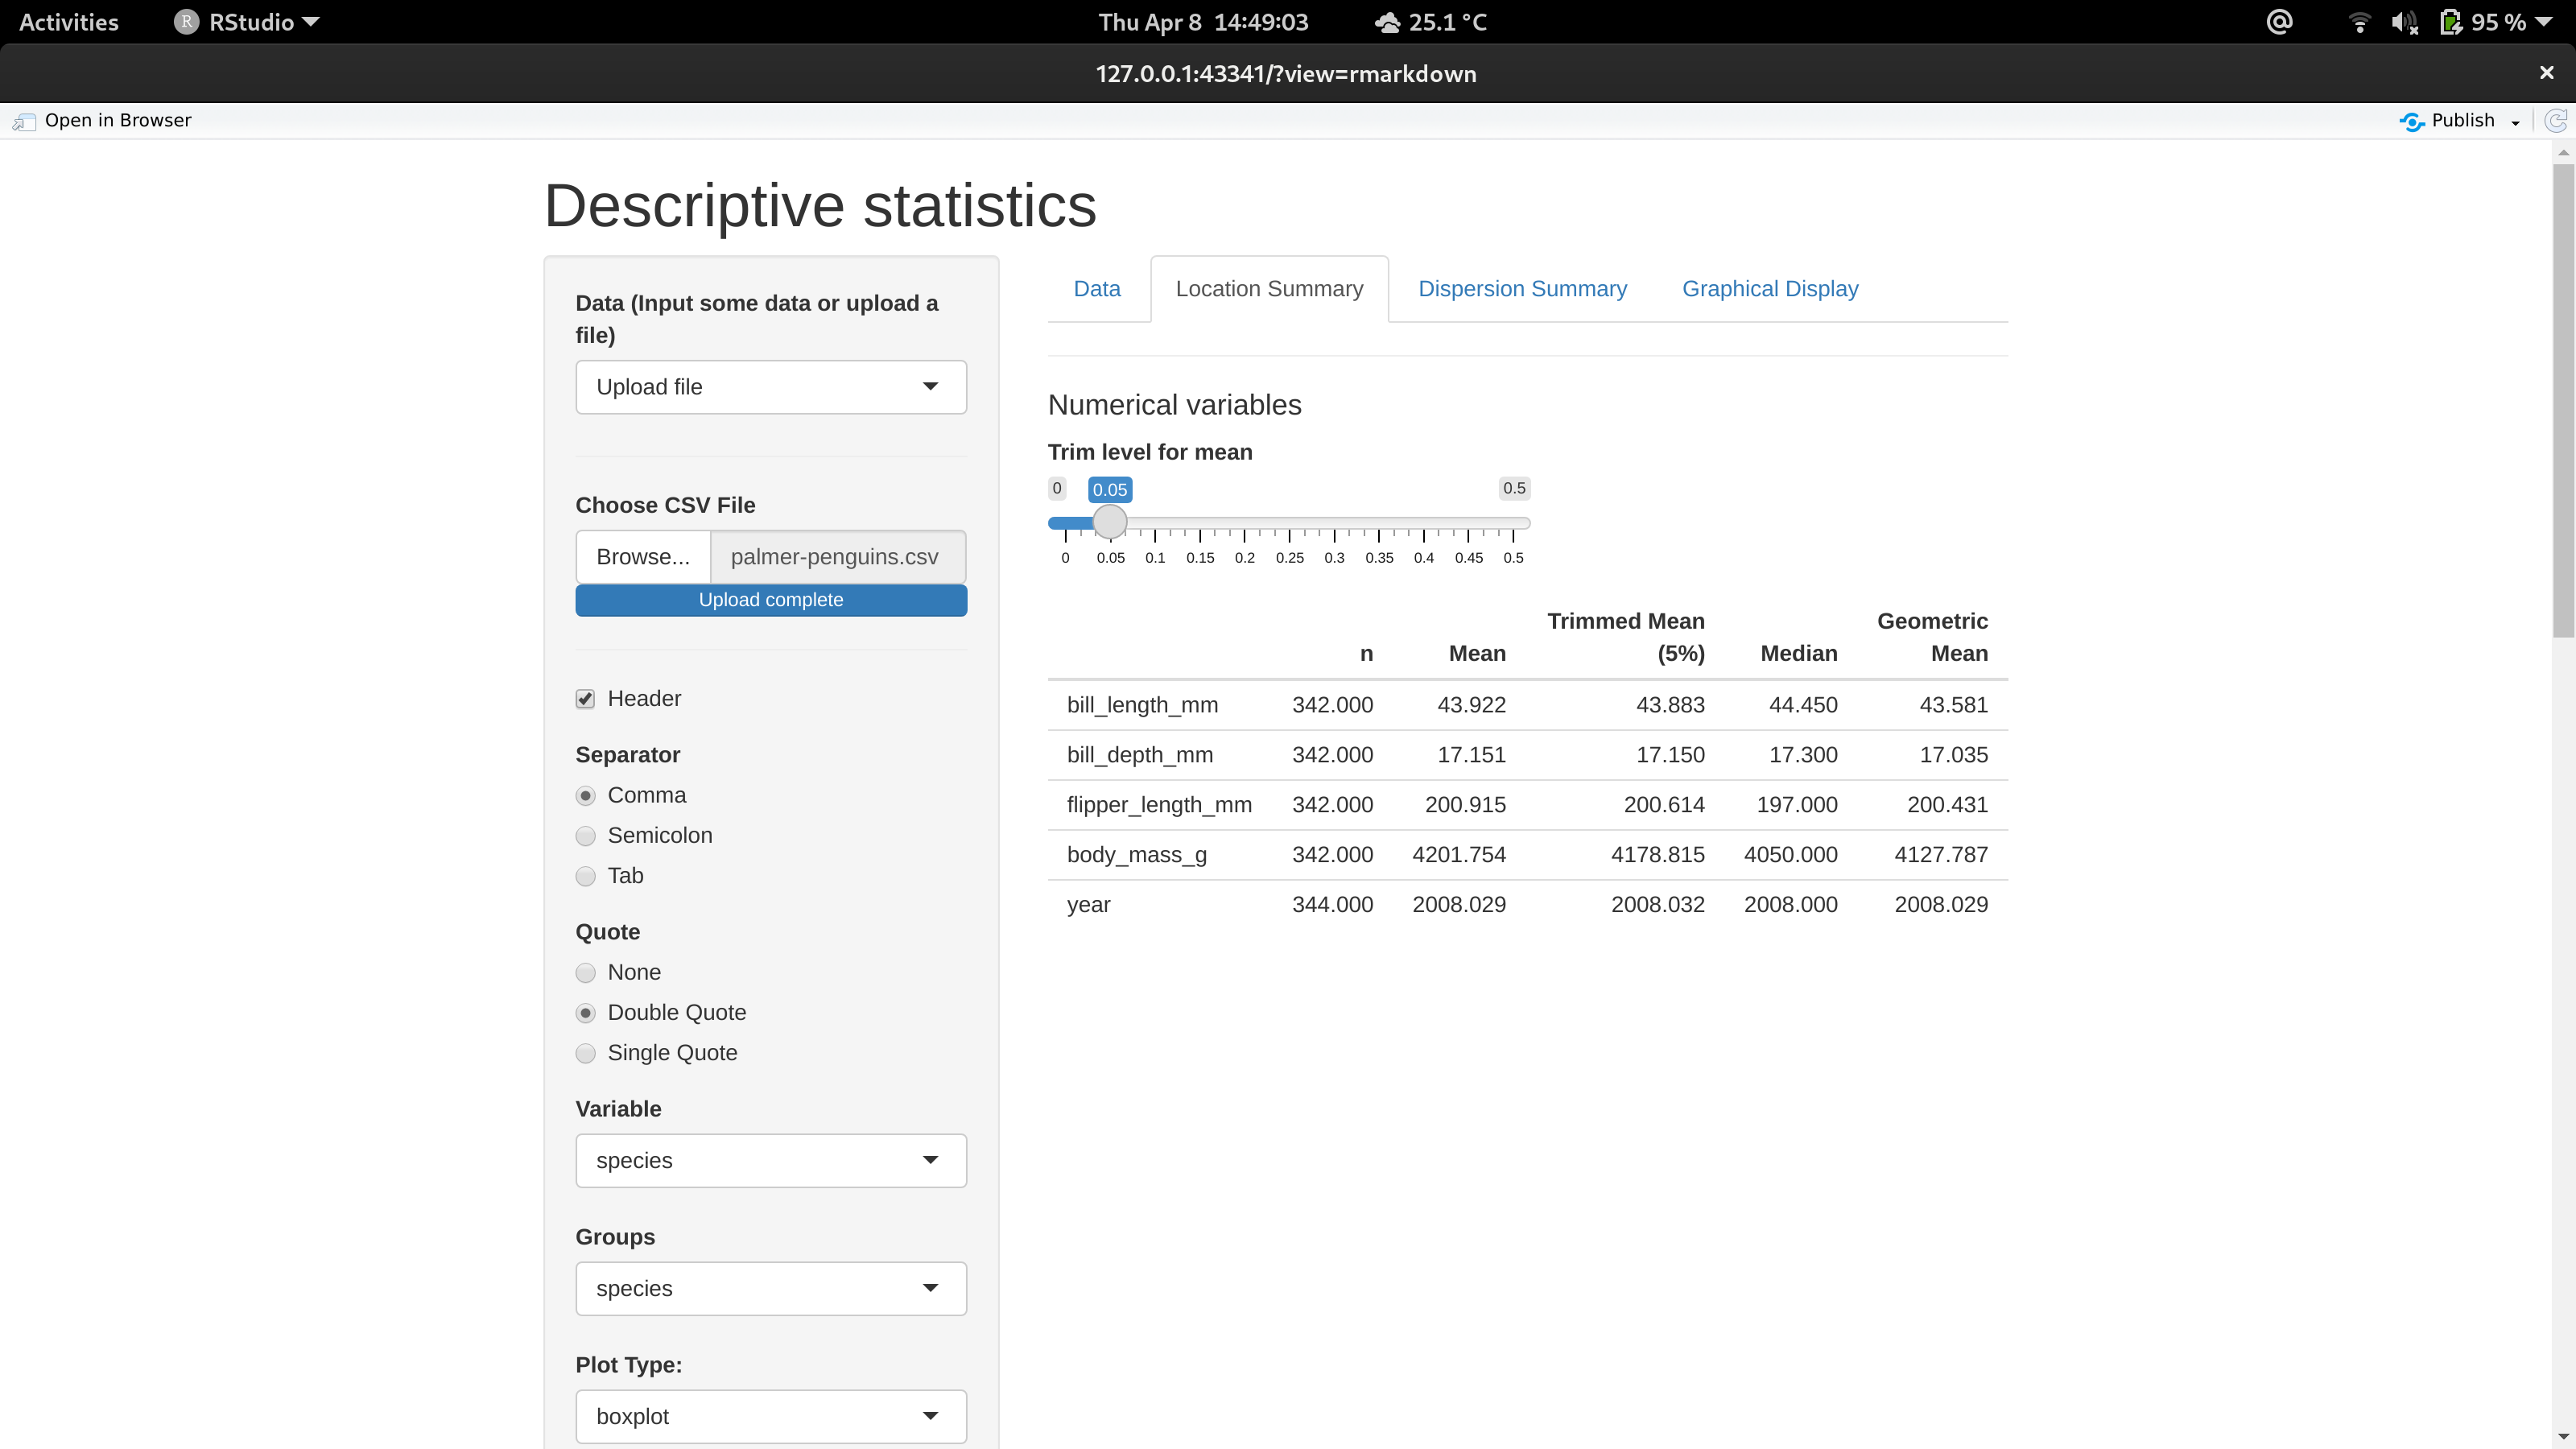
\includegraphics[width = \textwidth]{figures/Descriptive_2}
  \caption{Descriptive Statistics Web-page}\label{fig:DS2}
\end{figure}

\subsection{Inference}



A chi-square test (Snedecor and Cochran, 1983) can be used to test if the variance of a population is equal to a specified value. This test can be either a two-sided test or a one-sided test. The two-sided version tests against the alternative that the true variance is either less than or greater than the specified value. The one-sided version only tests in one direction. The choice of a two-sided or one-sided test is determined by the problem. For example, if we are testing a new process, we may only be concerned if its variability is greater than the variability of the current process. 


\subsection{Two Sample $t$-test}
The two-sample $t$-test (Snedecor and Cochran, 1989) is used to determine if two population means are equal. A common application is to test if a new process or treatment is superior to a current process or treatment.

There are several variations on this test.

- The data may either be paired or not paired. By paired, we mean that there is a one-to-one correspondence between the values in the two samples. That is, if $X_1, X_2, \ldots, X_n$ and $Y_1, Y_2,\ldots, Y_n$ are the two samples, then $X_i$ corresponds to $Y_i$. For paired samples, the difference $X_i-Y_i$ is usually calculated. For unpaired samples, the sample sizes for the two samples may or may not be equal. The formulas for paired data are somewhat simpler than the formulas for unpaired data.

- The variances of the two samples may be assumed to be equal or unequal. Equal variances yields somewhat simpler formulas, although with computers this is no longer a significant issue.

- In some applications, you may want to adopt a new process or treatment only if it exceeds the current treatment by some threshold. In this case, we can state the null hypothesis in the form that the difference between the two populations means is equal to some constant $\mu_1-\mu_2 =\delta_0$ where the constant is the desired threshold.



\subsection{Variance}

$H_0: \frac{\sigma^2_1}{\sigma^2_2} = 1$ versus $H_1: \frac{\sigma^2_1}{\sigma^2_2} \neq 1$

\subsection{Proportion}

$H_0: p_1 -p_2 = p_0$ versus $H_1: p_1-p_2 \neq p_0$


\subsection{Dependent $t$-test for paired samples}

This test is used when the samples are dependent; that is, when there is only one sample that has been tested twice (repeated measures) or when there are two samples that have been matched or ``paired''. This is an example of a paired difference test. The t statistic is calculated as
\[
    t = \frac{\bar{X}-\mu_0}{s_D/\sqrt{n}}
\]
where $\bar{X}$ are the average and $s_D$ standard deviation of the differences between all pairs. The pairs are e.g. either one person's pre-test and post-test scores or between-pairs of persons matched into meaningful groups (for instance drawn from the same family or age group: see table). The constant μ0 is zero if we want to test whether the average of the difference is significantly different. The degree of freedom used is $n-1$, where $n$ represents the number of pairs. 

\input{regression}
%\input{results}
\section*{Conclusions}

In this paper, we have outlined a framework for designing a web-based, modular, extensible system which reproduces user actions into \R code. We believe that the development strategies we’ve outlined can and should be applied to other software systems, as each of these characteristics aids in the ease-of-use and functionality of the overall product. Although we present them in the context of an introductory statistics application, these ideas are generalizable and we hope that they will gain traction in many other modern software systems.

Since the code is available and these are {\tt .Rmd} files. They can be used as a standalone application.

%\input{supporting}
\section*{Acknowledgments}
The authors are grateful for the software

\nolinenumbers

% Either type in your references using
% \begin{thebibliography}{}
% \bibitem{}
% Text
% \end{thebibliography}
%
% or
%
% Compile your BiBTeX database using our plos2015.bst
% style file and paste the contents of your .bbl file
% here. See http://journals.plos.org/plosone/s/latex for 
% step-by-step instructions.
% 
\begin{comment}
\begin{thebibliography}{10}

\bibitem{bib1}
Conant GC, Wolfe KH.
\newblock {{T}urning a hobby into a job: how duplicated genes find new
  functions}.
\newblock Nat Rev Genet. 2008 Dec;9(12):938--950.

\bibitem{bib2}
Ohno S.
\newblock Evolution by gene duplication.
\newblock London: George Alien \& Unwin Ltd. Berlin, Heidelberg and New York:
  Springer-Verlag.; 1970.

\bibitem{bib3}
Magwire MM, Bayer F, Webster CL, Cao C, Jiggins FM.
\newblock {{S}uccessive increases in the resistance of {D}rosophila to viral
  infection through a transposon insertion followed by a {D}uplication}.
\newblock PLoS Genet. 2011 Oct;7(10):e1002337.

\end{thebibliography}
\end{comment}


\end{document}

